\documentclass[12pt,fleqn]{article}
\setlength{\parindent}{0pt}
\usepackage{graphicx}
\usepackage{listings}
\usepackage[latin5]{inputenc}
\setlength{\parskip}{8pt}
\setlength{\parsep}{0pt}
\setlength{\headsep}{0pt}
\setlength{\topskip}{0pt}
\setlength{\topmargin}{0pt}
\setlength{\topsep}{0pt}
\setlength{\partopsep}{0pt}
\setlength{\mathindent}{0cm}

\begin{document}
Ders 5

Bir cizginin formulunu iki duzlemin kesisimi olarak gorduk, fakat bu
sekilde bir tanim cogunlukla bir cizgiyi tanimlamak icin en rahat / uygun
yol degildir, cunku elinizde bazi denklemler var, bunlari cozmekle ugrasmak
lazim, vs. 

Soyle bir yontem daha iyi olmaz mi? Cizgi uzerinde bir nokta hayal edelim,
ve bu noktanin, her zaman adiminda, cizgimizin oldugu yerlerden gectigini
dusunelim. Bu tur denklemlere parametrik denklem ismi veriliyor. 

Ornek

Cizgi uzerinde iki nokta verelim. 

\[ Q_0 = (-1,2,2) \]

\[ Q_1 = (1,3,-1) \]

Guzel, bu iki nokta var ama otekilerini nasil tanimlariz? Bu iki noktatinin
arasinda, sonrasinda, oncesinde olan tum noktalar da cizgiye dahildir. 

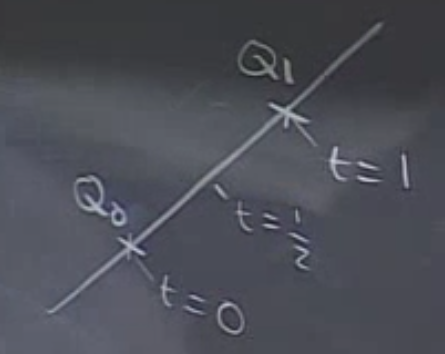
\includegraphics[height=4cm]{5_1.png}

Zaman araliklarini oyle dusunelim ki zaman indeksi sifir ($t=0$)
noktasinda, cizgi $Q_0$ uzerinde, tek birim adim atildiginda ($t=1$)  $Q_1$
uzerinde, gibi. O zaman yarim birim zamanda tam iki nokta ortasinda. 

Boylece cizgiyi temsil etmenin yolu onu $t$ bazinda hareket eden noktanin
gectigi yerler olarak tanimlamak. Bu temsilin en basit hali eger hareket
sabit hizda olursa olur. 

$t$ anindaki pozisyon $Q(t)$ nedir? 

Sorunun cevabini soyle vermeye baslayabiliriz: $\vec{Q_0Q(t)}$ vektoru
$\vec{Q_0Q_1}$ birbiriyle ortalidir. Bu oranti neye esittir? 

Bu oran $t$'ye esittir. O zaman

\[ \vec{Q_0Q(t)} = t \ \vec{Q_0Q_1}  \]

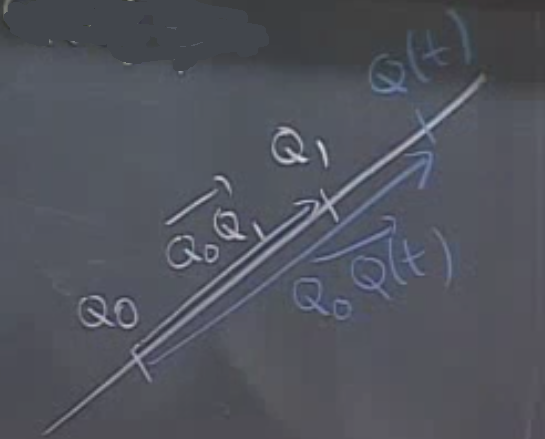
\includegraphics[height=4cm]{5_2.png}

O zaman iddia ediyorum ki bu formulu kullanarak ornegimizdeki hareket eden
noktanin yer formulunu bulabilirim.

\[ \vec{Q_0Q(t)} = t \ <2,1,-3>  \]

Simdi cizgi uzerinde hareket eden noktanin formulu $Q(t)$'yi su sekilde
temsil edelim

\[ Q(t) = <x(t),y(t),z(t)> \]

O zaman

\[ x(t) + 1 = t \ 2 \]

\[ y(t) - 2 = t \]

\[ z(t) - 2 = -3t \]

Usttekiler, alttaki su formun acilimindan ibaret aslinda

\[ Q(t) = Q_0 + t \ \vec{Q_0Q_1}  \]

Ustteki uc formul bu derste gordugumuz ilk parametrik cizgi
formulu. Formulun parcalari olan $x(t),y(t),z(t)$ sadece $t$'nin
fonksiyonudurlar, ve hep $t$ ile bir katsayinin carpimi + bir sabit
formundadirlar. $t$'nin katsayilari cizgi uzerindeki vektor hakkinda bilgi
verir, ve sabitler ise $t=0$ aninda nerede oldugumuzu gosteren baslangic
degerleridirler. 

Uygulama - Bir Duzlem ile Kesisme

Duzlem $x+2y+4z=7$. Cizgi biraz onceki formul olsun. Kesisme var midir, var
ise nerededir? 

Once su soruyu soralim kendimize. $x+2y+4z=7$ duzlemine gore, 
$Q_0 =
(-1,2,2)$ ve $Q_1 = (1,3,-1)$ noktalari duzlemin

\begin{enumerate}
   \item Ayni tarafinda
   \item Farkli taraflarinda
   \item Bir tanesi duzlem uzerinde
   \item Karar veremiyorum
\end{enumerate}

Cevaplayin. 

$Q_0$ ve $Q_1$ noktalarini duzlem formulunun sol tarafina sokariz. $Q_0$
icin sonuc $>7$, duzlem uzerinde degil, $Q_1$ icin sonuc $<7$, yine duzlem
uzerinde degil. Peki noktalar duzlemin hangi tarafinda? Ters tarafinda,
cunku biri $<7$, oteki $>7$ sonuc verdi. Bir duzlem uzayi iki yari-parcaya
(halfspace) ayirir ve noktalar bu ayri parcalardadirlar. Dogru cevap 2. 

Uygulamamizda cevaplanmayan bir soru daha var. Kesisme noktasi neresi?
$Q(t)$ nedir? Soyle

\[ x(t) + 2y(t) + 4z(t) \]

\[ = (-1+2t) + 2(2+t) + 4(2-3t) \]

Basitlestirelim

\[ = -8t + 11 \]

Bu formulu $7$ ile karsilastiralim cunku $Q(t)$ nin duzlem uzerinde oldugu
an $-8t + 11 = 7$ oldugu andir. Cebirsel olarak $t$'yi elde edebiliriz,
sonuc $t=1/2$. Bu degeri $Q(t)$'ye koyarsak

\[ Q(\frac{1}{2}) = (0,\frac{5}{2},\frac{1}{2}) \]

Kesisim noktasi esitligin sagindaki degerdir.

Yani eger cizginin parametrik denklemini biliyorsak, onu duzlem formulune
sokariz, ve kesisimin hangi noktada oldugunu hemen hesaplayabiliriz. 

Simdiye kadar gorduklerimizden parametrik denklemlerin cizgileri temsil
etmek icin iyi bir yontem olduklari belli olmustur herhalde. Bunun otesinde
parametrik denklemler uzaydaki herhangi bir egri (curve), herhangi bir
gidisati, yolu (trajectory) temsil etme kabiliyetine de sahiptir. 

Genel baglamda soylemek gerekirse, parametrik denklemleri uzayda icinde ya
duzlem uzerindeki herhangi (arbitrary) bir hareketi temsil etmek icin
kullanabiliriz.

Cycloid (Yuvarlanma Egrisi)

$a$ yari capindaki bir tekerlek yerde (x-ekseninde) donerek ilerliyor, $P$ bu
tekerlegin dis ceperinde (rim) bir nokta, baslangic noktasi 0 uzerinde. Ne
olur? Daha detayli olarak sormak gerekirse $P$ noktasinin hareketini
$t$'nin bir fonksiyonu $x(t),y(t)$ olarak hesaplayabilir miyiz?

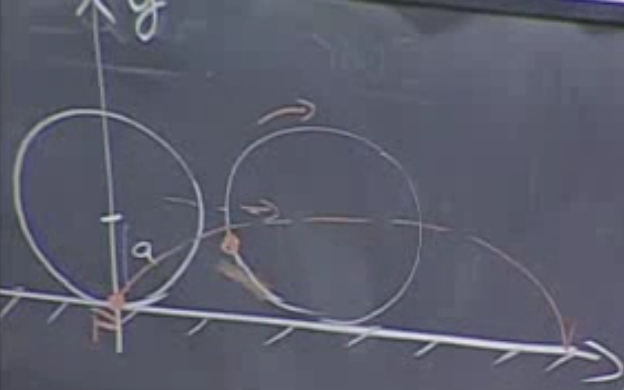
\includegraphics[height=4cm]{5_3.png}

[x-ekseni biraz saga yatik cikmis ama bu video kamerasinin acisi
yuzunden]. Bu ornegi bir bisikletin tekerligine takilmis bir isigin,
bisiklet gece giderken ortaya cikartabilecegi goruntuyu dusunurek te hayal
edebiliriz. Yani hem donus hareketi var, hem de yatay olarak duz bir gidis
hareketi var.

Bu $P$ noktasinin gidis yolunu hesaplamak icin tekerlegin ne kadar hizli
dondugu onemli mi? Hayir degil. Yavas ta hizli da dondursek, $P$ ayni
noktalardan gececektir. 

Bu problemde en onemli faktor zaman degil, mesafe, tekerlegin ne kadar
mesafe katettigi. Ya da daha bile iyisi, mesafe ile donus birbirine
baglantili olduguna gore, ve problemdeki en cetrefil, girift olus donme
(rotation) olduguna icin, belki de tekerlegin ne kadar dondugunu gosteren
bir aci degeri, bu buyuklugu kullanirsak belki daha faydali olacak. Pek cok
degisik temsil yontemi olabilir, fakat aciya gore parametrize edersek en
temiz formulu elde etmek mumkun olur. O zaman $x(t),y(t)$ yerine
$x(\theta),y(\theta)$ kullanalim. 

Yani $x(\theta),y(\theta)$ ile tekerlegin ne kadar donmus oldugunu
belirleyen $\theta$ aci uzerinden tanimli bir fonksiyon kullanalim. 

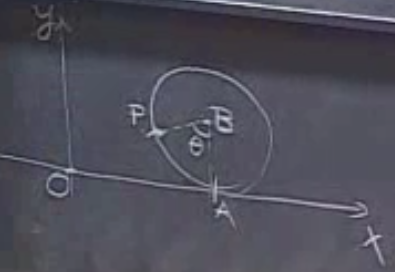
\includegraphics[height=4cm]{5_4.png}

Tekerlegin nerede oldugu bilgisini ise $\vec{OP}$ vektoru ile temsil
edebilirim. Buradaki tek problem vektor $\vec{OP}$ hakkinda hic bir sey
bilmiyorum. Ama belki daha basit vektorler hakkinda bir seyler
biliyorumdur. Mesela $\vec{AB}$ basit gibi duruyor, ayni sekilde $\vec{OA}$
fena degil, $\vec{BP}$ ayni sekilde. Peki $\vec{OP}$'yi bu daha basit
vektorler uzerinden temsil edemez miyim? Edebilirim. 

\[ \vec{OP} = \vec{OA} + \vec{AB} + \vec{BP}  \]

O zaman bu basit vektorleri hesaplayabilirsem, daha zor olan $\vec{OP}$'yi
de hesaplarim. 

\[ \vec{OA} = <a\theta, 0> \]

Niye? Vektorun $y$ bileseni sifir, bu bariz. 

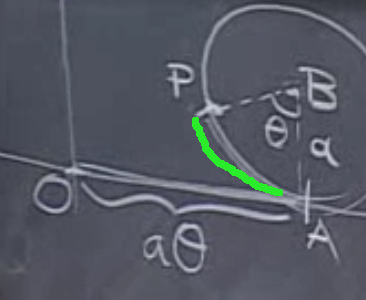
\includegraphics[height=3cm]{5_5.png}

Peki niye $a\theta$? Eger kayma, bosta donme gibi seyler yok ise, bu
tekerlegin dis cemberinin katettigi donus / geldigi nokta (ustte yesil ile
isaretli), tekerlegin gittigi yer mesafesi ile aynidir. Bu yuzeylerden
birinin kavisli, digerinin duz olmasi bu gercegi degistirmez. Yesil ile
isaretli dis cember parcasinin $a\theta$ ile hesaplandigini basit
matematikten biliyoruz (eger $\theta$ radyan biriminde ise tabii, zaten bu
sebeple -isleri basitlestirdigi icin- matematikte hep radyan birimi
kullanilir). 

$\vec{AB}$ daha kolay, $x$ bileseni sifir, $y$ yonune yaricap kadar
gitmis. 

\[ \vec{AB} = <0, a> \]

En son vektor $\vec{BP}$ biraz daha zor. Bu vektor hakkinda neler
biliyoruz? Buyuklugunu yani $|\vec{BP}|$'yi biliyoruz ve dikey eksen ile
$\theta$ kadar bir aci olusturdugunu biliyoruz. Daha yakindan bakarsak

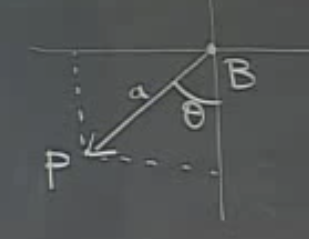
\includegraphics[height=2cm]{5_6.png}

\[ \vec{BP} = <-asin(\theta), -acos(\theta)> \]

Simdi ekleme asamasina geldik. 

\[ \vec{OP} = <a\theta - asin(\theta), a-acos(\theta)> \]

Ve nihayet cevabimizi bulduk. Cunku 

\[ \vec{OP} = 
<
\underbrace{a\theta - asin(\theta)}_{x(\theta)}, 
\underbrace{a-acos(\theta)}_{y(\theta)}
> \]

Bu problemi modellerken zihnimizde olusan, istifade ettigimiz �ekil �u:

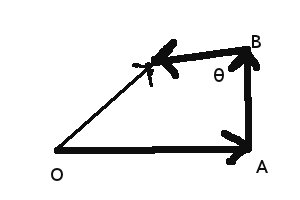
\includegraphics[height=2cm]{cycloid-lines.png}

��nk� vektor toplaminin geometrik olarak nasil isledigini biliyoruz, ve
eksik kalacak tek parca, basit toplamayla elde edecegimiz aradigimiz
parametrik vektor olacak. Bu yontemi secmemizin bir diger sebebi ustteki
parcalarin hepsinin basit hesaplanabiliyor olmasi, her uc vektor icin de
yaricap $a$ mutlaka bir hesaba dahil, ve bu yaricap hic degismeyen bir sey,
dolayisiyla modellememizi basitlestiriyor. Yine benzer bir sebeple $\theta$
$\vec{OP}$ vektorunun x-ekseniyle olusturdugu aci degil, $\vec{BP}$'nin
y-ekseniyle olusturdugu a��. Boylece onun uzerinden ve $a$ ile uc vektoru
hizli bir sekilde hesaplayabiliyoruz. 

Ayrica modellemede parametre $t$ degil, $\theta$. Bu mantikli, degisimi ile
tum vektor ogelerini bir sekilde etkileyen (ayri formuller uzerinden tabii)
her dis degisken bir parametre olarak kullanilabilir.  

Simdi gizemli bir noktayi inceleyelim. Tekerlegin donmesi sonucu takip
edilen noktanin yere degip, tekrar yukari ciktigi anda, olusan takip
cizgisi ne sekildedir? Bilgisayar grafigine bakalim; 

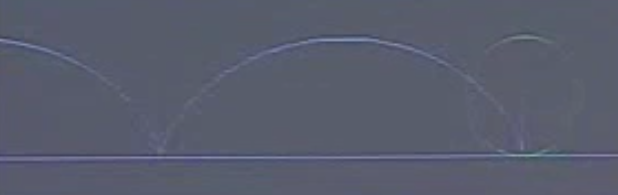
\includegraphics[height=4cm]{5_7.png}

Sekil sunlardan hangisidir? 

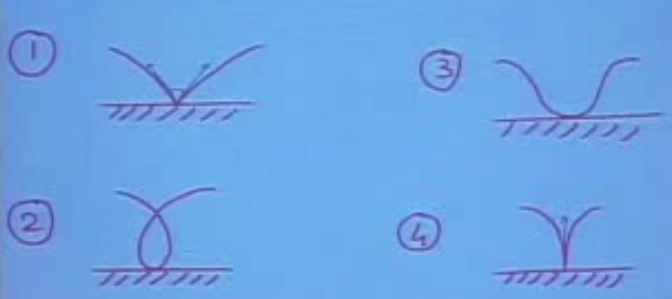
\includegraphics[height=4cm]{5_8.png}

Bu cevabi vermenin en iyi yolu, formullerimizi kullanmak. 

Formulleri basitlestirmek icin eger $a=1$ alirsak, 

\[ x(\theta) = \theta - sin(\theta) \]

\[ y(\theta) = 1 - cos(\theta) \]

Simdi yaklasiksal olarak dusunmeye ugrasalim. Cok kucuk $\theta$ icin
$sin(\theta) \approx \theta$ ve $cos(\theta) \approx 1$. Bunlari
$x(\theta), y(\theta)$ icinde kullanirsak, biri 0, oteki 1 cikacak, bunlar
pek net sonuclar degiller. Demek ki bize daha iyi yaklasiksal (approximate)
teknikler gerekiyor. 

Tek Degiskenli Calculus dersinde Taylor Yaklasiksallamasi ogretilir. 

Taylor Yaklasiksallamasi

Kucuk $t$ degerleri icin 

\[ f(t) \approx f(0) \]

Bu kabaca bir yaklasiksallamadir tabii ki. Biraz daha iyisi icin, eger $t$
kadar degisim olursa, bu degisimin su sekilde eklenebilecegini farzederiz.

\[ f(t) \approx f(0) + tf'(0)\]

Biraz daha iyisi icin

\[ f(t) \approx f(0) + tf'(0) + \frac{t^2}{2}f''(0)\]

Buna istedigimiz kadar devam edebiliriz

\[ f(t) \approx f(0) + tf'(0) + \frac{t^2}{2}f''(0) + \frac{t^3}{6}f'''(0)\]

Bu teknigi simdi kullanalim

\[ sin(\theta) \approx \theta - \frac{\theta^3}{6} \]

\[ cos(\theta) \approx 1 - \frac{\theta^2}{2} \]

O zaman

\[ x(\theta) \approx \theta - (\theta  - \frac{\theta^3}{6}) 
\approx \frac{\theta^3}{6} 
\]

\[ y(\theta) \approx 1 - (1  - \frac{\theta^2}{2}) 
\approx \frac{\theta^2}{2} 
\]

Bu degerlerden hangisi $\theta$ kucuk iken daha buyuk? $y(\theta)$. Yani
$|x| << |y|$. Daha net bir sayi icin bu iki buyuklugun oranina bakabiliriz,
bu bize bir egim bilgisi verecektir. 

\[ \frac{y}{x} = \frac{\theta^3/6}{\theta^2/2 } = 
\frac{3}{\theta} \to \infty, \ \ \theta \to 0
\]

Yani $\theta$ sifira yaklasirken egim neredeyse sonsuz, takip ettigimiz
nokta saga, sola neredeyse hic hareket etmiyor, neredeyse tum hareket dikey
sekilde. Demek ki ustte 4. sekil dogru cevap. 

Problem 1E-4

$(0,1,2)$ ve $(2,0,3)$ noktalarindan gecen cizgi duzlem $x + 4y + z = 4$'i
nerede keser? 

Cevap

A ve B noktalari uzerinden bir yon, yani bir vektor hesaplayabiliriz, 
$\vec{AB}
= <2,-1,1>$. Sonra bu vektorun katlari kadar, $t$ adimi atarak, baslangic
noktasindan sonsuza kadar giden cizginin parametrik formulunu buluruz, yani
$A + \vec{AB} \ t$. 

\[ x = 0 + 2t = 2t \]

\[ y = 1 - t \]

\[ z = 2 + t \]

Parametrik formulu duzlem formulunde yerine koyalim. 

\[ (2t) + 4(1-t) + (2+t) = 4 \]

Cozunce $t=2$ cikar. Bunu parametrik formulde yerine koyunca $(4,-1,4)$
kesisim noktasini elde ederiz. 

Problem 1E-5 

$(1,1,-1)$ noktasindan gecen cizgi $x+2y - z = 3$ duzlemine diktir. Bu
cizgi $2x - y + z = 1$ duzlemini hangi noktada keser? 

Cevap

Kesisim hesabi icin cizginin parametrik denklemini bulmamiz lazim. Eger bu
cizgi ilk duzleme dik ise, o duzlemin normali ``yonunde'' gitmektedir, o
zaman elimizde bir yon var, bir de baslangic noktasi var. O noktadan,
normal yonunde $t$ adimi atmayi kodlayacagiz (birinci duzlem ile kesisme
onemli degil). 

\[ x(t) = 1 + t \]

\[ y(t) = 1 + 2t \]

\[ z(t) = -1 -t \]

Simdi bu cizginin ikinci duzlemle kesistigi soylendigine gore, sunun dogru
olmasi gerekir

\[ 2(1+t) - (1+2t) + (-1-t) = 1 \]

Yani parametrik denklemin ogelerini teker teker ikinci duzlemin icine
koymus oluyoruz. Ustteki denklemi cozunce $t=-1$ cikacak. Bunu alip
parametrik denkleme geri koyarsak, elde edilen nokta $(0,-1,0)$
noktasidir [ders cevaplarinda 0,1,0 deniyor, bu yanlis]. 




\end{document}

